\documentclass[10pt,a4paper,twocolumn]{article}
\usepackage[subtle,mathdisplays=normal]{savetrees}
\usepackage[T1]{fontenc}
\usepackage[utf8]{inputenc}
\usepackage{anysize, longtable}
\usepackage{amsthm, amsfonts, amsmath, amssymb, booktabs, float}
\usepackage{sectsty, csquotes, xcolor, xspace, setspace, listings}
\usepackage{graphicx, tabularx, changepage, multirow, subcaption}
\usepackage{algorithm, algpseudocode, multicol, cuted}
\usepackage[hidelinks,bookmarksdepth=3]{hyperref}
\usepackage[capitalise]{cleveref}
\usepackage[inline]{enumitem}
\usepackage[english]{babel}
\usepackage{microtype}
\usepackage{libertinus}
\usepackage[scale = 0.85]{plex-mono}
\usepackage[maxbibnames=99]{biblatex}
\usepackage{titlesec}
\usepackage{tikz}

\input{draft.tex}

\usetikzlibrary{fit, shapes.geometric, positioning, shapes.misc, calc, arrows.meta, patterns, backgrounds, decorations, decorations.markings, decorations.pathreplacing, shadows, hobby}

\makeatletter

\theoremstyle{plain}
\newtheorem{theorem}{Theorem}
\newtheorem{lemma}{Lemma}

\theoremstyle{definition}
\newtheorem{definition}{Definition}
\newtheorem{example}{Example}

\theoremstyle{remark}
\newtheorem*{note}{Note}
\newtheorem*{remark}{Remark}

\newcommand{\inlinecode}[1]{\lstinline[basicstyle=\ttfamily,columns=fixed]$#1$}
\lstset{basicstyle=\setstretch{0}\small\ttfamily,breaklines=true,columns=fixed,captionpos=b,xleftmargin=0.5cm}

\newlength{\offsetpage}
\newenvironment{widepage}[1][2cm]{
  \setlength{\offsetpage}{#1}
  \begin{adjustwidth}{-\offsetpage}{-\offsetpage}
  \addtolength{\linewidth}{2\offsetpage}
}{\end{adjustwidth}}

\algnewcommand{\IIf}[1]{\State \algorithmicif\ #1\ \algorithmicthen}
\algnewcommand{\IElse}[1]{\algorithmicelse\ #1}
\algnewcommand{\EndIIf}{\unskip\ \algorithmicend\ \algorithmicif}

\addbibresource{biblio.bib}

\allowdisplaybreaks
\marginsize{2.0cm}{2.0cm}{1.25cm}{1.25cm}
\setcounter{tocdepth}{2}
\setlist[itemize]{topsep=0pt, partopsep=0pt, parsep=0pt, itemsep=\parskip}
\setlist[enumerate]{topsep=0pt, partopsep=0pt, parsep=0pt, itemsep=\parskip}
\titlespacing*{\paragraph}{0pt}{0.5\baselineskip}{0.5\baselineskip}
\captionsetup[figure]{aboveskip=5pt}
\captionsetup[subfigure]{aboveskip=3pt}

\title{Evaluating the Negotiation Abilities of Large Language Models Using Game Play}
\author{Roland Bernard, 19598, \inlinecode{rolbernard@unibz.it}}
\date{June 2025}

\def\maketitle{
\begin{strip}
  \begin{adjustwidth}{5mm}{5mm}
    \noindent{\LARGE\bfseries \@title\par}
    \vskip 1em
    \noindent{\large \@author\par}
    \vskip 1em
    \noindent{\small \@date\par}
    \vskip 1em
  \end{adjustwidth}
\end{strip}
}
\renewenvironment{abstract}{
  \vskip 1em
  \begin{quote}
  {\normalsize \abstractname\par}
  \small
}{
  \end{quote}
  \vskip 1em
}

\makeatother

\input{tikzfigures/defs.tex}

\begin{document}

\maketitle

\begin{abstract}
Lorem ipsum dolor sit amet, consectetur adipiscing elit, sed do eiusmod tempor incididunt ut labore et dolore magna aliqua. Ut enim ad minim veniam, quis nostrud exercitation ullamco laboris nisi ut aliquip ex ea commodo consequat. Duis aute irure dolor in reprehenderit in voluptate velit esse cillum dolore eu fugiat nulla pariatur. Excepteur sint occaecat cupidatat non proident, sunt in culpa qui officia deserunt mollit anim id est laborum
\end{abstract}

\section{Introduction} \label{introcudction}

In the last several years we have experienced a dramatic evolution in the capabilities of Large Language Models (LLMs), which now demonstrate remarkable performance across a wide range of Natural Language Processing (NLP) tasks. These include not only text generation or summarization but also complex reasoning. As a result, these models are increasingly integrated into various applications. However, traditional methods for evaluating LLMs, which often rely on static benchmark datasets, have significant limitations. Most importantly, these benchmarks are susceptible to data contamination, where test data may have been included in the massive training corpora of the models \cite{magar-schwartz-2022-data}. Furthermore, they fail to assess the abilities of models in interactive scenarios that more closely reflect real-world human interactions with the models.

Dialogue games have been proposed as a tool for LLM evaluation addressing these shortcomings. The \inlinecode{clembench} framework, in particular, offers a structured approach to this by introducing the concept of a \inlinecode{clemgame}, which is an interactive, goal-oriented dialogue game played between two LLM agents, arbitrated by a programmatic game master \cite{chalamalasetti-etal-2023-clembench}. Such a setup allows for the evaluation of nuanced capabilities such as strategic reasoning, instruction following, and language grounding in a dynamic but still controlled environment.

This project leverages the \inlinecode{clembench} framework to introduce a new game, Deal or No Deal (DoND), designed to probe a set of capabilities not extensively covered by existing \inlinecode{clemgames}. Specifically, this new game tries to evaluate negotiation skills, ability to express and understand preferences, and the ability to compromise. In DoND, players must communicate to reach a mutually beneficial agreement on the division of a set of items, each holding different values for each player. Aside from negotiation, the game also challenges the LLM's ability to adhere to rules, such as using a specific syntax for final proposals. Furthermore, it requires the LLMs be capable of maintaining conversational grounding by reasoning about the items as well as its own and the other players preferences as stated in the dialogue.

The primary question this project attempts to answer then it how various state-of-the-art LLMs perform in this new \inlinecode{clemgame} specifically designed to test their negotiation, strategic communication, and rule-following abilities.

To answer this question, the objectives of this project were the following:
\begin{enumerate*}
    \item To design and implement a new \inlinecode{clemgame}, based on the DoND negotiation task, including with different game modes to create cooperative, semi-competitive, and competitive scenarios.
    \item To select and apply appropriate evaluation metrics to assess LLM performance, focusing on rule adherence, the rate of agreement, and the quality of the outcomes.
    \item To conduct an experiment using a diverse set of recent open- and closed-weight LLMs to analyse their performance across multiple languages, specifically English, German, and Italian.
    \item To identify and discuss the strengths and weaknesses of the evaluated LLMs within this negotiation setting, providing mainly quantitative but also some qualitative insights.
\end{enumerate*}

The remainder of this report is structured as follows:
\Cref{related} reviews related work in LLM evaluation, dialogue games, and AI for negotiation.
\Cref{experiment} details the experimental design, including the game mechanics, instance generation process, dialogue flow, evaluation metrics, and the overall setup.
\Cref{results} presents and analyses the results of the experiments, offering both a quantitative breakdown and some qualitative discussion of model behaviours.
Finally, \Cref{conclusion} concludes with a summary of the findings and discusses the contributions and limitations of the project, highlighting possible avenues for future research.


\section{Related Work} \label{related}

The architecture of prominent LLMs, which is primarily based on the Transformer model \cite{vaswani2017attention}, has enabled a significant increase in scale and performance of language models. Further, the development from foundational models, which were primarily trained on next-token prediction, such as GPT 3, to instruction-tuned and chat-optimized models, like GPT 3.5 and GPT 4, has also marked a significant shift. Techniques like Reinforcement Learning from Human Feedback (RLHF) have been used to align these models more closely with user intent, making them more adept at following instructions and engaging in coherent, multi-turn conversations \cite{ouyang2022training}. This project specifically evaluates these newer, chat-optimized models, as their interactive nature makes them more fitting candidates for playing dialogue games.

The \inlinecode{clembench} framework \cite{chalamalasetti-etal-2023-clembench,beyer2024clembench} serves as the foundation for this project. Its purpose is to enable the systematic and reproducible evaluation of LLMs as conversational agents through game play. The framework is structured such that a programmatic game master controls the game flow, presents instructions and game states to LLM players, and parses their responses. This allows for automated scoring and isolates the evaluation to the abilities of the LLMs to understand and act within the constraints of the game, rather than their ability to generate unconstrained text.

Existing \inlinecode{clemgames} in the benchmark evaluate a wide range of different abilities. For instance, the taboo game tests concept description and semantic understanding under constraints, while the drawing and reference games test a form of multimodal grounding through character-based grids. The DoND game presented in this project complements these by introducing a direct test of negotiation, compromise, and strategic reasoning based on conflicting objectives and incomplete information. These capabilities are central to many real-world interactions but were not the primary focus of prior games included in the benchmark. Other related work in evaluating LLMs in interactive environments also includes frameworks that use LLMs as referees and focus on more open-ended social interactions \cite{li2023beyond,zhou2024sotopia}. In contrast, \inlinecode{clembench} focuses on structured, automatically scorable games, providing a possibly more easily understandable and objective lens.

The problem of dividing resources between agents with different preferences is a classic topic in game theory, and has been formalized by John Nash in 1950 \cite{nash1950equilibrium,nash1950bargaining}. The DoND game is such a multi-issue bargaining task, where agents must find a point in the solution space that is mutually agreeable. Note however that unlike in the standard semi-competitive setting, in the cooperative setting also evaluated in this project, the task is purely cooperative, and so the agreement should be trivial for rational agents if given full information.

Research on AI agents in negotiation also has a long history, though much of it has focused on agents that communicate using symbolic actions or pre-defined logical forms rather than unrestricted natural language. However, a number of key papers have used the DoND setting to train AI systems. This project is substantially influenced by those works. \cite{lewis2017deal} and \cite{he2018decoupling} used this and similar negotiation tasks to train agents using a combination of supervised and reinforcement learning. More recently, \cite{liao2024efficacy} used the same DoND game to investigate the efficacy of fine-tuning through self-play. They found that iterative training via filtered behaviour cloning could dramatically improve model performance. However, they concluded that the increased performance was not due to improved high-level strategy, but due to improvements in rule-following and the ability to reach agreements.

This project fundamentally differs from these works in its objective. The goal here is not to train or fine-tune models. Instead, the DoND game is used as an instrument for zero-shot evaluation of pre-trained, general-purpose LLMs, assessing their inherent out-of-the-box negotiation capabilities. This way the project benchmarks the baseline performance of these models and identifies their intrinsic strengths and weaknesses in a negotiation context.


\section{Experiment} \label{experiment}


This section of the report discusses the methodology used for running the experimental evaluation. It follows a detailed description of the game rules, the used evaluation metrics, and some general information about the experimental setup.


\subsection{The Game}




\subsection{Evaluation Metrics}




\subsection{Experimental Setup}




\section{Results} \label{results}


In this section of the report, the results of the experiments will be discussed. The main focus is on the analysis of quantitative results, but this section also contains some qualitative analysis and discussions.


\subsection{Quantitative Analysis}

\begin{figure}[ht]
  \centering
  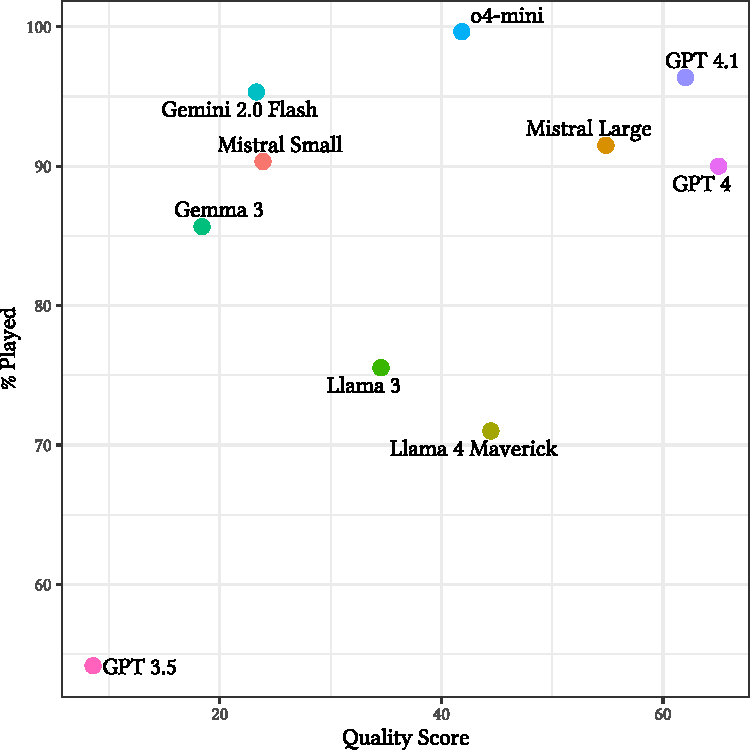
\includegraphics[width=\linewidth]{figures/playedquality.pdf}
  \caption{Summarized evaluation results for each model. The y-axis indicates the percentage of played, i.e., not aborted, games. The x-axis represents the average quality score obtained when considering only played games.}
  \label{fig:playedquality}
\end{figure}


\begin{figure}[ht]
  \centering
  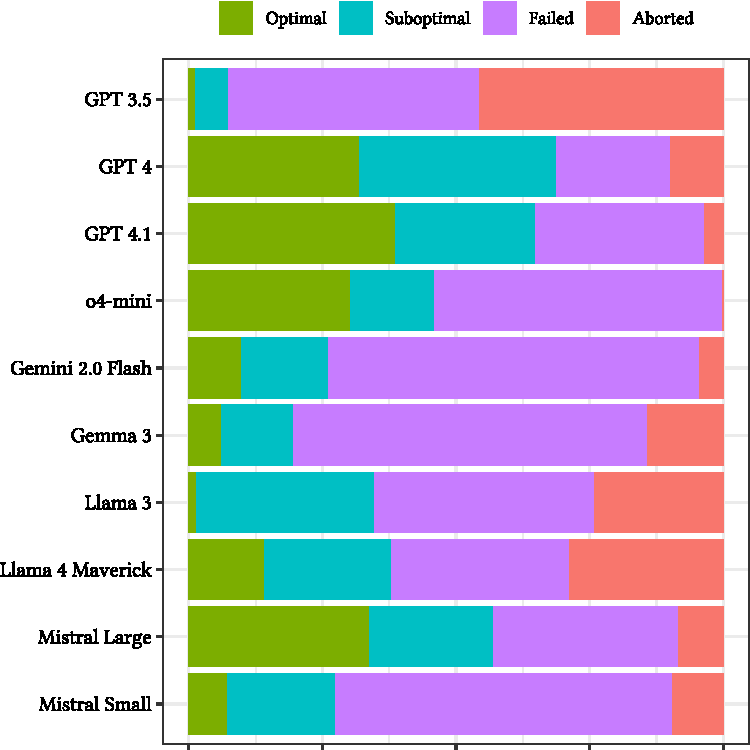
\includegraphics[width=\linewidth]{figures/outcome.pdf}
  \caption{Percentage of games that ended with a specific game outcome during the evaluation of different models. All results for the two game modes and three languages have been averaged together for this plot.}
  \label{fig:outcome}
\end{figure}


\begin{table*}[ht]
  \scriptsize
  \begin{widepage}
    \centering
    \addtolength{\tabcolsep}{-0.2em}
    \begin{tabular}{lllcccccccccc}
      \hline
      Mode & Lang. & Metric & GPT 3.5 & GPT 4 & GPT 4.1 & o4-mini & Gemini 2.0 & Gemma 3 & Llama 3 & Llama 4 & Mistral Large & Mistral Small \\
      \hline
      semi & en & Clemscore & 0 & 61 & 69 & 44 & 42 & 20 & 0 & 49 & 38 & 24 \\
      semi & en & \% Played & 32 & 100 & 98 & 100 & 98 & 82 & 14 & 86 & 72 & 80 \\
      semi & en & \% Agreement & 7 & 78 & 74 & 48 & 47 & 32 & 0 & 70 & 61 & 35 \\
      semi & en & \% Optimal & 0 & 30 & 51 & 36 & 24 & 10 & 0 & 30 & 39 & 18 \\
      semi & en & Quality Score & 0 & 61 & 70 & 44 & 42 & 24 & 0 & 57 & 53 & 30 \\
      semi & en & Avg. \# Messages & 3.3 & 7.9 & 7.1 & 4.3 & 6.9 & 7 & 10 & 6.6 & 8.5 & 6.5 \\
       \hline
      semi & de & Clemscore & 9 & 43 & 59 & 41 & 8 & 9 & -- & 26 & 60 & 21 \\
      semi & de & \% Played & 66 & 81 & 98 & 100 & 89 & 82 & -- & 74 & 100 & 92 \\
      semi & de & \% Agreement & 16 & 68 & 70 & 43 & 12 & 12 & -- & 41 & 69 & 30 \\
      semi & de & \% Optimal & 6 & 32 & 35 & 37 & 4 & 7 & -- & 22 & 43 & 9 \\
      semi & de & Quality Score & 14 & 53 & 61 & 41 & 9 & 11 & -- & 36 & 60 & 23 \\
      semi & de & Avg. \# Messages & 3.3 & 7 & 6.3 & 4.1 & 8.6 & 6.2 & -- & 6.9 & 6 & 5.2 \\
      \hline
      semi & it & Clemscore & 4 & 50 & 49 & 17 & 15 & 15 & -- & 19 & 64 & 26 \\
      semi & it & \% Played & 51 & 93 & 95 & 100 & 96 & 90 & -- & 66 & 100 & 98 \\
      semi & it & \% Agreement & 13 & 62 & 59 & 20 & 19 & 20 & -- & 33 & 72 & 35 \\
      semi & it & \% Optimal & 0 & 36 & 34 & 9 & 10 & 9 & -- & 12 & 48 & 8 \\
      semi & it & Quality Score & 7 & 53 & 51 & 17 & 16 & 17 & -- & 29 & 64 & 26 \\
      semi & it & Avg. \# Messages & 3.8 & 7.4 & 6 & 5.1 & 6.7 & 6.1 & -- & 5.7 & 6.2 & 5.4 \\
      \hline
      coop & en & Clemscore & 3 & 74 & 65 & 57 & 31 & 25 & 29 & 48 & 26 & 26 \\
      coop & en & \% Played & 56 & 100 & 100 & 100 & 92 & 90 & 60 & 78 & 77 & 86 \\
      coop & en & \% Agreement & 11 & 83 & 67 & 60 & 37 & 31 & 60 & 74 & 39 & 37 \\
      coop & en & \% Optimal & 0 & 36 & 43 & 44 & 11 & 11 & 0 & 18 & 22 & 12 \\
      coop & en & Quality Score & 6 & 74 & 65 & 57 & 33 & 27 & 48 & 62 & 35 & 31 \\
      coop & en & Avg. \# Messages & 2.9 & 7.8 & 6.7 & 4.7 & 7.1 & 6.4 & 9.1 & 6.7 & 8.9 & 6 \\
      \hline
      coop & de & Clemscore & 9 & 37 & 65 & 51 & 16 & 15 & 27 & 20 & 66 & 9 \\
      coop & de & \% Played & 86 & 63 & 98 & 98 & 96 & 76 & 86 & 60 & 100 & 86 \\
      coop & de & \% Agreement & 16 & 67 & 70 & 58 & 21 & 26 & 44 & 40 & 71 & 14 \\
      coop & de & \% Optimal & 3 & 22 & 44 & 31 & 8 & 0 & 2 & 23 & 39 & 0 \\
      coop & de & Quality Score & 11 & 59 & 66 & 52 & 17 & 20 & 32 & 33 & 66 & 10 \\
      coop & de & Avg. \# Messages & 2.2 & 6.6 & 6.6 & 4.1 & 10.1 & 6 & 9.1 & 6.2 & 6 & 5.5 \\
      \hline
      coop & it & Clemscore & 3 & 84 & 50 & 39 & 15 & 10 & 24 & 26 & 46 & 24 \\
      coop & it & \% Played & 35 & 100 & 89 & 100 & 98 & 94 & 90 & 62 & 100 & 100 \\
      coop & it & \% Agreement & 12 & 92 & 62 & 46 & 20 & 15 & 39 & 52 & 53 & 30 \\
      coop & it & \% Optimal & 0 & 50 & 31 & 22 & 0 & 4 & 2 & 10 & 27 & 2 \\
      coop & it & Quality Score & 7 & 84 & 57 & 39 & 16 & 11 & 27 & 42 & 46 & 24 \\
      coop & it & Avg. \# Messages & 7.2 & 7.4 & 6.2 & 4.5 & 7 & 6.4 & 9.7 & 5.9 & 6.4 & 5.1 \\
      \hline
    \end{tabular}
  \end{widepage}
  \caption{Detailed breakdown of the results for each game mode, language, and model combination across multiple metrics. The best result in each row is indicated in bold.}
  \label{tab:results}
\end{table*}


\subsection{Qualitative Analysis}




\subsection{Overall Performance Summary}




\section{Conclusion} \label{conclusion}

In conclusion, this project successfully designed, implemented, and utilized a new \inlinecode{clemgame}, Deal or No Deal, to conduct a rigorous evaluation of the negotiation capabilities of ten prominent LLMs. The findings reveal that while the latest generation of models, such as GPT-4.1, show a commendable ability to follow the game rules accurately and engage in superficially coherent negotiations, they still lack deep strategic reasoning. Models often fail to adapt their strategy to the specific goals of the game mode, falling back on generic negotiation patterns. Performance is highly variable across models, with some models clearly outperforming the rest.

Still, this work still has several limitations that could be potential avenues for future research. For example, only ten different models were tested in this project. A wider array of models could provide a more complete picture of the landscape, and reveal some underlying patterns explaining the differences in performance. Introducing human players to negotiate against LLMs could also provide a more realistic assessment of their capabilities. Further, all the game instances evaluated here were relatively small, i.e., few items and short dialogues, to ensure tractability. Performance might differ on more complex negotiation tasks. Another limitation of this work is the limited selection of languages. A broader linguistic analysis would therefore be beneficial. Future work could also explore the evaluation of the strictly competitive game mode. While its exclusion was a considered design choice based on methodological difficulties, it means the performance of the models in purely adversarial scenarios remains untested. The qualitative analysis performed for this project was also quite limited. Developing methods to automatically categorize the types of errors LLMs make, e.g., role confusion, logical contradiction, etc., would also enable more scalable qualitative analysis. Furthermore, future work could focus on a more fine-grained analysis of the negotiation strategies employed by the LLMs, perhaps by trying to identify specific tactics. Finally, this project used a single, fixed set of prompts. The impact of different prompting strategies on LLM performance was not explored. 



\printbibliography

\end{document}
